
\section{Visão geral}

Vulkan é uma API gráfica de baixo nível em que a aplicação declara explicitamente cada recurso que os shaders vão ler, como esses recursos são agrupados, quando são atualizados e como a CPU e a GPU se sincronizam. Para o UV mapping dinâmico e procedural, isso significa responder a quatro perguntas: onde ficam as coordenadas UV, como o tempo chega ao shader a cada quadro, como a textura e o sampler são expostos e onde cada cálculo é feito.

A Figura~\ref{fig:pipeline-vulkan} mostra a arquitetura da implementação. Em azul estão os dados e recursos da aplicação; em verde, os estágios do pipeline e os shaders; em laranja, os mecanismos de sincronização; em roxo, o descriptor set, o Render Pass e seus attachments; em amarelo, as operações específicas de UV mapping. As setas contínuas indicam o sentido em que um dado trafega, com o rótulo do que é transmitido. As setas tracejadas em laranja indicam dependências de sincronização. Os grupos tracejados reúnem recursos do mesmo tipo. O arquivo-fonte do diagrama, gerado com Graphviz, está em \texttt{diagrama/pipeline\_vulkan.dot}. O restante do capítulo descreve cada parte a partir da implementação entregue (\texttt{código/src/VulkanApp.cpp}), que renderiza o modelo \texttt{Duck.glb} em cinco modos selecionáveis pelas teclas 1 a 5.

\begin{figure}[p]
    \centering
    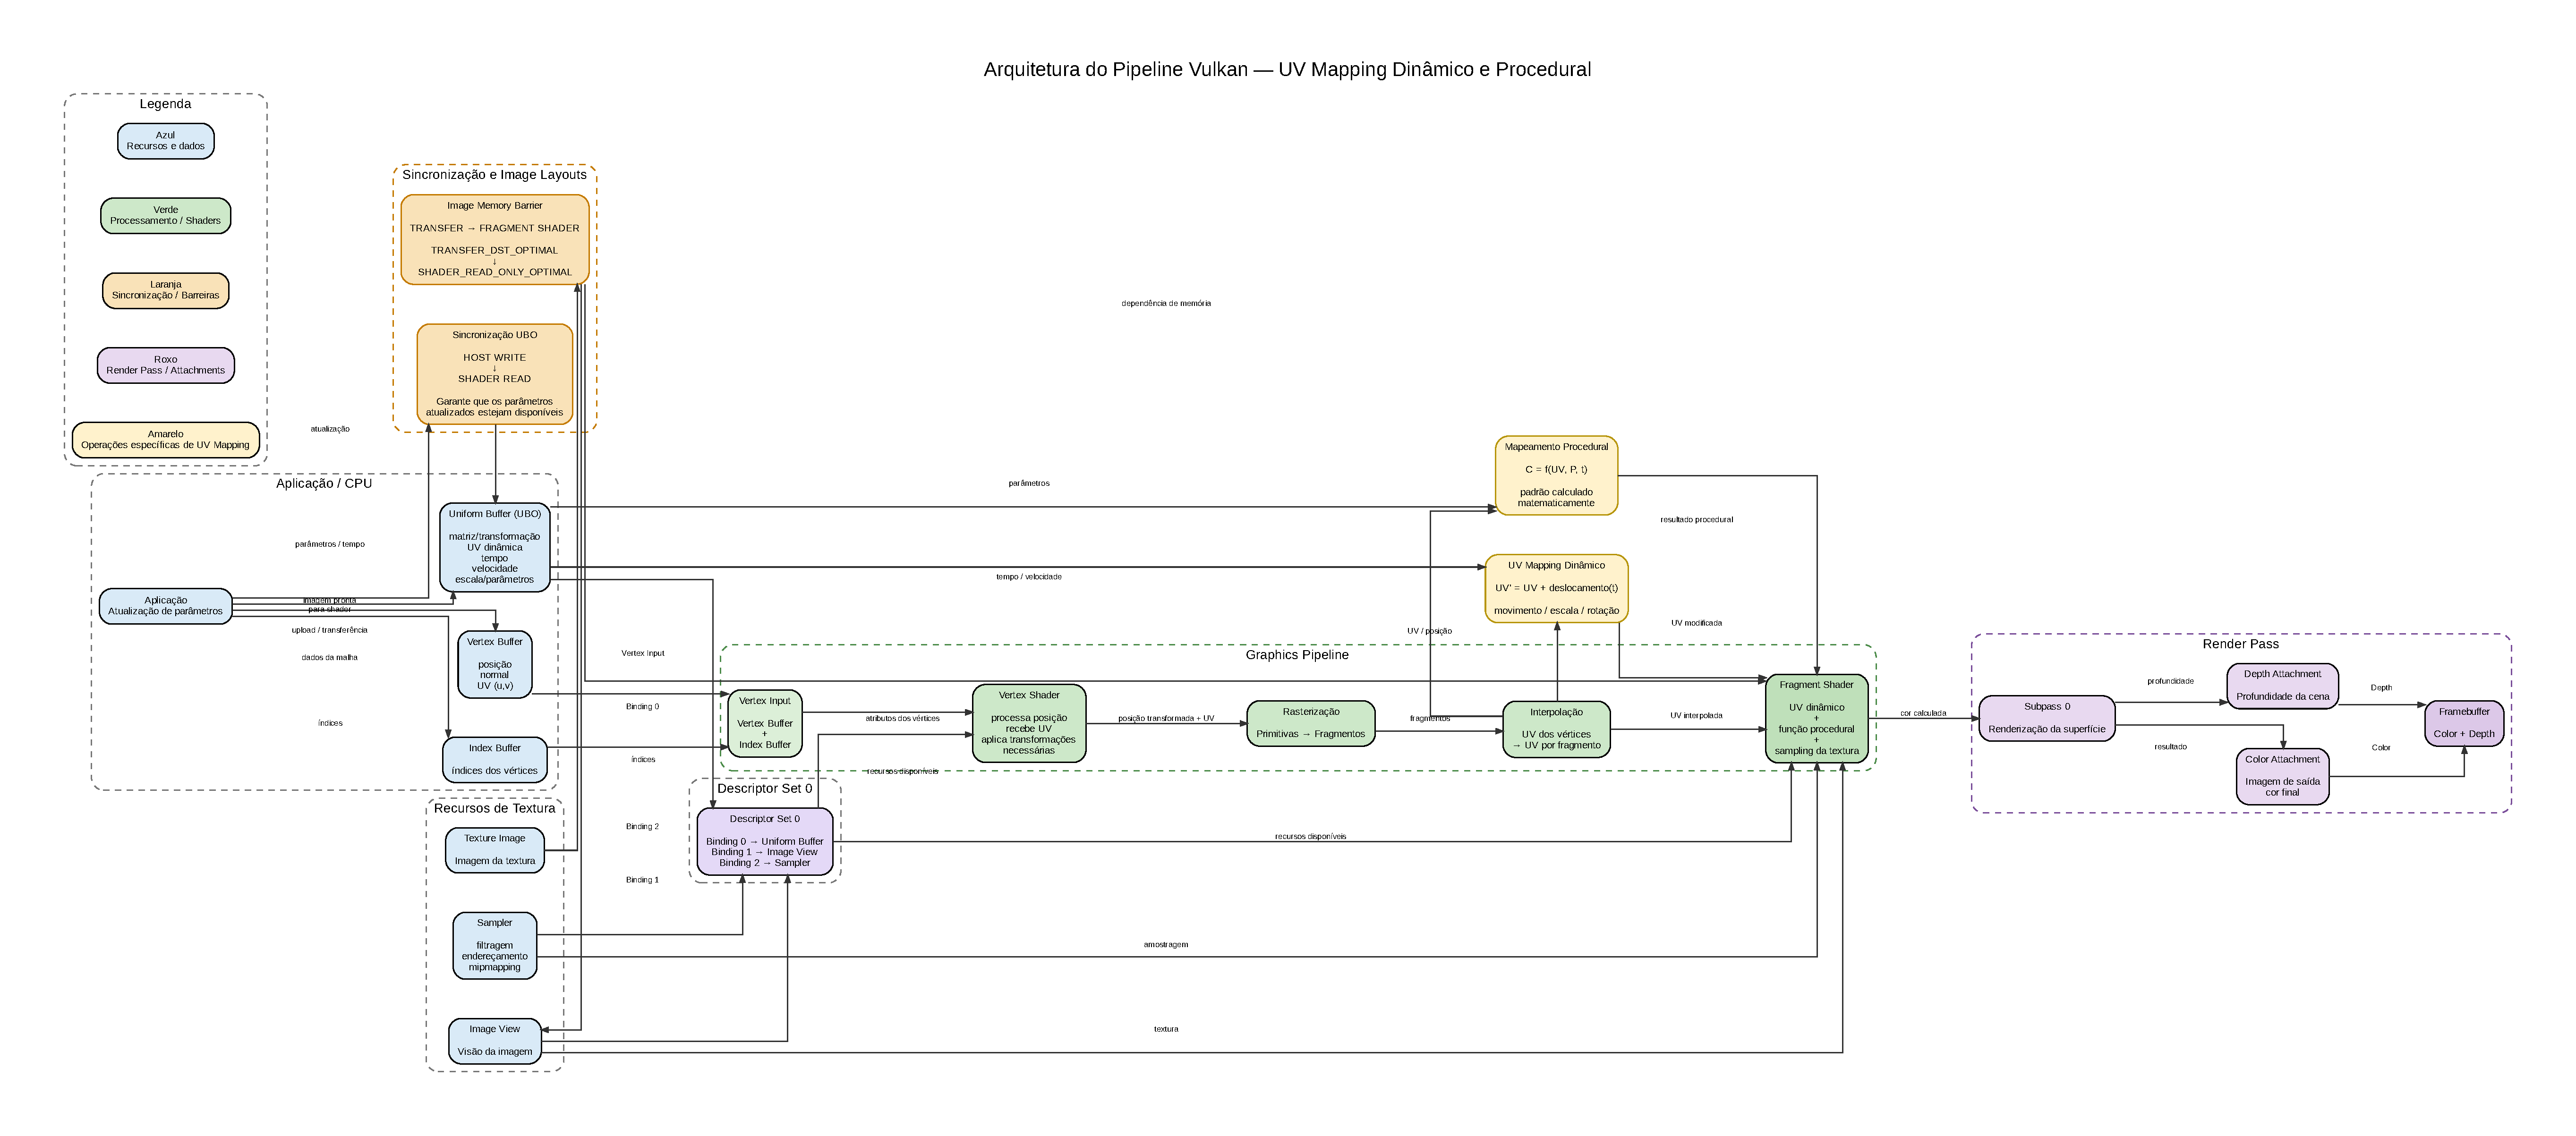
\includegraphics[width=\textwidth,height=0.80\textheight,keepaspectratio]{diagrama/pipeline_vulkan.pdf}
    \caption{Arquitetura do pipeline Vulkan aplicada ao UV mapping dinâmico e procedural, conforme a implementação.}
    \label{fig:pipeline-vulkan}
    \vspace{4pt}
    \small
    \begin{tabular}{@{}l@{\hspace{6pt}}l@{\hspace{14pt}}l@{\hspace{6pt}}l@{}}
    \colorbox[HTML]{D9EAF7}{\strut\hspace{1.2em}} & dados e recursos &
    \colorbox[HTML]{CDE8C9}{\strut\hspace{1.2em}} & estágios e shaders \\
    \colorbox[HTML]{F9E2B8}{\strut\hspace{1.2em}} & sincronização &
    \colorbox[HTML]{E4D9F7}{\strut\hspace{1.2em}} & descriptor set e render pass \\
    \colorbox[HTML]{FFF2CC}{\strut\hspace{1.2em}} & operações de UV mapping &
    \(\longrightarrow\) / \textcolor[HTML]{C47A00}{\(\dashrightarrow\)} & fluxo de dados / sincronização \\
    \end{tabular}
\end{figure}

\section{Recursos usados pela técnica}

\begin{table}[H]
\centering
\caption{Recursos Vulkan da implementação e o papel de cada um no UV mapping.}
\label{tab:recursos-vulkan}
\small
\begin{tabular}{p{2.5cm}p{4.3cm}p{3.5cm}p{3.5cm}}
\toprule
\textbf{Recurso} & \textbf{Configuração} & \textbf{Conteúdo} & \textbf{Atualização} \\
\midrule
Vertex Buffer & \texttt{DEVICE\_LOCAL}, enviado via \textit{staging buffer} & 2.399 vértices de 32 bytes (posição, normal, UV) & Uma vez, na inicialização \\
Index Buffer & \texttt{DEVICE\_LOCAL}, \texttt{UINT32} & 12.636 índices (4.212 triângulos) & Uma vez \\
Uniform Buffer & \texttt{HOST\_VISIBLE | HOST\_COHERENT}, mapeado permanentemente; um por imagem da swapchain & 208 bytes: \(M\), \(V\), \(P\), \texttt{time}, \texttt{mode} & A cada quadro (\texttt{memcpy}) \\
Imagem de textura & \texttt{R8G8B8A8\_SRGB}, \(512\times512\), \texttt{mipLevels = 1} & Cor base do modelo & Uma vez \\
Sampler & \texttt{LINEAR}, \texttt{REPEAT} nos três eixos, anisotropia no máximo do dispositivo & Filtragem e endereçamento & Imutável \\
\bottomrule
\end{tabular}
\end{table}

O Vertex Buffer usa um único binding (0), com \textit{stride} de 32 bytes e taxa por vértice. Cada vértice tem três atributos: posição em \texttt{location 0} (\texttt{R32G32B32\_SFLOAT}, offset 0), normal em \texttt{location 1} (\texttt{R32G32B32\_SFLOAT}, offset 12) e UV em \texttt{location 2} (\texttt{R32G32\_SFLOAT}, offset 24). O Index Buffer é uma lista contínua de inteiros de 32 bits, três por triângulo.

A divisão segue a frequência de atualização de cada dado. Geometria e textura nunca mudam e ficam em memória \texttt{DEVICE\_LOCAL}, a mais rápida para a GPU ler. Os parâmetros que mudam a cada quadro ficam em memória visível pela CPU. O formato \texttt{SRGB} faz a GPU converter a cor para o espaço linear na leitura, de modo que a filtragem e a iluminação operam sobre valores lineares. A textura é formada por três objetos \cite{vulkan}:
\begin{itemize}
    \item a \texttt{VkImage}, que guarda os texels;
    \item a \texttt{VkImageView}, que define como interpretá-los;
    \item o \texttt{VkSampler}, que define como lê-los.
\end{itemize}
Para o UV dinâmico, o sampler é tão importante quanto o shader: o modo \texttt{REPEAT} permite que \(u + 0{,}10\,t\) continue lendo a textura depois de ultrapassar 1, e a filtragem \texttt{LINEAR} evita que o deslocamento lento da textura ``salte'' de um texel para o próximo.

\section{Fluxo de dados entre os estágios}

\begin{table}[H]
\centering
\caption{Estágios do pipeline: o que entra, o que sai e quais recursos são compartilhados.}
\label{tab:estagios}
\small
\begin{tabular}{p{2.5cm}p{3.6cm}p{3.6cm}p{4.1cm}}
\toprule
\textbf{Estágio} & \textbf{Entra} & \textbf{Sai} & \textbf{Recursos usados} \\
\midrule
Aplicação (CPU) & Tempo do relógio, tecla do modo & \(M\), \(V\), \(P\), \texttt{time}, \texttt{mode} & Uniform Buffer da imagem atual \\
Vertex Input & Vertex e Index Buffers & Posição, normal e UV de cada vértice & Vertex Buffer (32 bytes por vértice), Index Buffer \\
Vertex Shader & Atributos do vértice, matrizes & \texttt{gl\_Position}, \texttt{fragUV}, \texttt{fragNormal} & Binding 0 (UBO) \\
Rasterização & Triângulos em espaço de recorte & Fragmentos com UV e normal interpolados (Eq.~\ref{eq:perspectiva}) & Depth attachment (teste de profundidade) \\
Fragment Shader & \texttt{fragUV}, \texttt{fragNormal}, \texttt{time}, \texttt{mode}, textura & Cor final (\texttt{outColor}) & Binding 0 (UBO), binding 1 (textura e sampler) \\
Saída de cor & Cor do fragmento & Pixel no color attachment & Color attachment, framebuffer, swapchain \\
\bottomrule
\end{tabular}
\end{table}

Dois recursos são compartilhados entre estágios: o Uniform Buffer, lido pelos dois shaders, e o depth attachment, escrito e testado durante a rasterização. A textura só é lida pelo fragment shader.

\section{Descriptor Sets e Bindings}

Um \textit{descriptor} é a forma como o Vulkan informa a um shader onde está um recurso. Os descriptors são agrupados em \textit{descriptor sets}, cujo formato é declarado por um \texttt{VkDescriptorSetLayout}. A implementação usa um único set (\texttt{set = 0}) com dois bindings, criados em \texttt{createDescriptorSetLayout}.

\begin{table}[H]
\centering
\caption{Layout do Descriptor Set 0 na implementação.}
\label{tab:descriptor-impl}
\small
\begin{tabular}{cp{4.4cm}p{3.0cm}p{4.6cm}}
\toprule
\textbf{Binding} & \textbf{Tipo} & \textbf{Estágios} & \textbf{Declaração GLSL} \\
\midrule
0 & \texttt{UNIFORM\_BUFFER} & Vertex e Fragment & \texttt{uniform Parameters \{...\} params} \\
1 & \texttt{COMBINED\_IMAGE\_SAMPLER} & Fragment & \texttt{uniform sampler2D baseTexture} \\
\bottomrule
\end{tabular}
\end{table}

O binding~0 é visível nos dois estágios porque o vertex shader usa as matrizes e o fragment shader usa \texttt{time} e \texttt{mode}. O binding~1 é declarado só para o fragment shader, o único que lê a textura. Restringir os \texttt{stageFlags} ao necessário informa ao driver quais estágios precisam enxergar cada recurso. São alocados tantos descriptor sets quantas são as imagens da swapchain, cada um apontando para o seu próprio Uniform Buffer. Assim, a CPU não sobrescreve o \texttt{time} de um quadro enquanto a GPU ainda lê o anterior. O set de cada imagem é ligado uma única vez, com \texttt{vkCmdBindDescriptorSets}, no command buffer daquela imagem.

\subsection{Do projeto à implementação}
\label{sec:projeto-impl}

O projeto inicial da arquitetura (feito antes da implementação, junto com o pseudocódigo em \texttt{pseudocodigo/}) previa três bindings: o Uniform Buffer (0), a imagem (\texttt{SAMPLED\_IMAGE}, 1) e o sampler (\texttt{SAMPLER}, 2), separados. Na implementação, imagem e sampler foram unidos em um \texttt{COMBINED\_IMAGE\_SAMPLER}. As duas formas são válidas, e a escolha depende de quantas texturas existem. Com uma textura e um sampler, o descriptor combinado é mais simples: um binding e uma escrita de descriptor a menos, e o GLSL usa \texttt{sampler2D} diretamente. A separação compensa quando muitas texturas compartilham as mesmas regras de filtragem, por exemplo em um material com cor, normal e rugosidade, em que um único \texttt{VkSampler} é reutilizado.

O Uniform Buffer também mudou. O projeto previa os campos \texttt{uvVelocity} e \texttt{uvScale}. A implementação os trocou por \texttt{time} e \texttt{mode} e deixou as velocidades como constantes no shader, porque elas não variam em tempo de execução. O campo \texttt{mode} seleciona qual dos cinco cálculos o fragment shader executa.

\subsection{Layout de memória do Uniform Buffer (std140)}

O GLSL usa o layout \texttt{std140} para blocos \texttt{uniform}, e a struct C++ precisa ter os mesmos deslocamentos em bytes. A implementação verifica isso em tempo de compilação com \texttt{static\_assert}:

\begin{verbatim}
struct UniformBufferObject {
    glm::mat4 model;       // offset   0
    glm::mat4 view;        // offset  64
    glm::mat4 projection;  // offset 128
    float     time;        // offset 192
    int32_t   mode;        // offset 196
    float     padding[2];  // total: 208 bytes
};
\end{verbatim}

Se um campo fosse reordenado na struct sem a mesma alteração no shader, o tempo seria lido como lixo e a animação pararia, sem nenhum erro de validação. A verificação transforma esse problema em erro de build.

\section{Push constants}

Push constants são uma segunda forma de enviar dados ao shader, sem buffer nem descriptor. Os valores são gravados diretamente no command buffer com \texttt{vkCmdPushConstants} \cite{vkpushconstants} e declarados no shader como \texttt{layout(push\_constant)}. O espaço é pequeno: o limite \texttt{maxPushConstantsSize} tem mínimo garantido de 128 bytes, ou 256 bytes em dispositivos com Vulkan~1.4 \cite{vkmapping,vklimits}. Em troca, a atualização dispensa memória mapeada e um buffer por quadro em execução.

Os dados que mais mudam no UV dinâmico são os candidatos ideais. O par \texttt{time} e \texttt{mode} ocupa 8 bytes; as três matrizes (192 bytes) não cabem no mínimo garantido. Com push constants, o shader e a aplicação ficariam assim:

\begin{verbatim}
layout(push_constant) uniform Animation { float time; int mode; } anim;

vkCmdPushConstants(cmd, pipelineLayout, VK_SHADER_STAGE_FRAGMENT_BIT,
                   0, sizeof(Animation), &anim);
\end{verbatim}

A implementação mantém tudo no Uniform Buffer por uma razão concreta. Os command buffers são gravados uma única vez, em \texttt{createCommandBuffers}, um por imagem da swapchain, e depois apenas reenviados. Como o valor de uma push constant fica gravado dentro do command buffer, usá-las exigiria regravá-lo a cada quadro. Com o Uniform Buffer, os command buffers continuam estáticos e só os 208 bytes do buffer mapeado são reescritos. Para uma versão seguinte, a divisão mais adequada é híbrida: matrizes no Uniform Buffer e \texttt{time}/\texttt{mode} em push constants, com o command buffer regravado por quadro. Essa é a abordagem mais comum em cenas que mudam continuamente, e o custo de gravar um único \textit{draw call} é desprezível.

\section{Render Pass e Subpass}

A implementação usa um Render Pass com um único subpass (Subpass~0), que desenha o modelo, e dois attachments:
\begin{itemize}
    \item \textbf{Color attachment} (formato da swapchain): é limpo no início (\texttt{LOAD\_OP\_CLEAR}), gravado no fim (\texttt{STORE\_OP\_STORE}) e entregue em \texttt{PRESENT\_SRC\_KHR} para ser exibido. Recebe a cor final do fragment shader.
    \item \textbf{Depth attachment} (\texttt{D32\_SFLOAT} ou o melhor formato disponível): é limpo a cada quadro e descartado no fim (\texttt{STORE\_OP\_DONT\_CARE}), porque a profundidade só serve para decidir a visibilidade dentro do próprio quadro.
\end{itemize}
Os dois attachments são ligados a um Framebuffer por imagem da swapchain. Um único subpass basta porque a técnica não precisa de pós-processamento: todo o UV mapping acontece no fragment shader do mesmo passo.

\section{Sincronização: barreiras, layouts e dependências}

\textbf{Transições de layout e barreiras da textura.} A textura passa por duas transições de layout, cada uma com uma \textit{image memory barrier}, criadas em \texttt{transitionImageLayout}:

\begin{table}[H]
\centering
\caption{Barreiras de memória da textura na implementação.}
\label{tab:image-barrier}
\small
\begin{tabular}{p{2.9cm}p{5.2cm}p{5.6cm}}
\toprule
\textbf{Campo} & \textbf{Barreira 1} & \textbf{Barreira 2} \\
\midrule
Recurso & Imagem da textura & Imagem da textura \\
Etapa anterior & \texttt{TOP\_OF\_PIPE} (nenhuma) & \texttt{TRANSFER} \\
Acesso anterior & nenhum & escrita de transferência \\
Etapa posterior & \texttt{TRANSFER} & \texttt{FRAGMENT\_SHADER} \\
Acesso posterior & escrita de transferência & leitura no shader \\
Layout anterior & \texttt{UNDEFINED} & \texttt{TRANSFER\_DST\_OPTIMAL} \\
Layout posterior & \texttt{TRANSFER\_DST\_OPTIMAL} & \texttt{SHADER\_READ\_ONLY\_OPTIMAL} \\
Motivo & Colocar a imagem no layout que aceita a cópia do staging buffer (\texttt{vkCmdCopyBufferToImage}). & Garantir que a cópia terminou e está visível antes da primeira amostragem; sem ela, o shader poderia ler uma textura parcialmente copiada. \\
\bottomrule
\end{tabular}
\end{table}

\textbf{Dependência do subpass e transições dos attachments.} As transições dos attachments são feitas pelo próprio Render Pass, sem barreiras explícitas, e sincronizadas por uma \texttt{VkSubpassDependency} de \texttt{VK\_SUBPASS\_EXTERNAL} para o Subpass~0:

\begin{table}[H]
\centering
\caption{Dependência do subpass e transições dos attachments.}
\label{tab:subpass-dep}
\footnotesize
\begin{tabular}{p{2.4cm}p{5.0cm}p{6.3cm}}
\toprule
\textbf{Campo} & \textbf{Color attachment} & \textbf{Depth attachment} \\
\midrule
Recurso & Imagem da swapchain & Imagem de profundidade \\
Etapa anterior & \texttt{COLOR\_ATTACHMENT\_OUTPUT} (quadro anterior) & \texttt{LATE\_FRAGMENT\_TESTS} (quadro anterior) \\
Acesso anterior & --- & escrita de profundidade \\
Etapa posterior & \texttt{COLOR\_ATTACHMENT\_OUTPUT} & \texttt{EARLY\_FRAGMENT\_TESTS} \\
Acesso posterior & escrita de cor & escrita de profundidade \\
Layout anterior & \texttt{UNDEFINED} & \texttt{UNDEFINED} \\
Layout no subpass & \texttt{COLOR\_ATTACHMENT\_OPTIMAL} & \texttt{DEPTH\_STENCIL\_ATTACHMENT\_OPTIMAL} \\
Layout final & \texttt{PRESENT\_SRC\_KHR} & \texttt{DEPTH\_STENCIL\_ATTACHMENT\_OPTIMAL} \\
Motivo & Não escrever na imagem antes de ela ser liberada pela apresentação anterior & Não limpar a profundidade enquanto o quadro anterior ainda a testa e grava \\
\bottomrule
\end{tabular}
\end{table}

O layout anterior \texttt{UNDEFINED} indica que o conteúdo antigo pode ser descartado, o que é correto porque os dois attachments são limpos no início do passo.

\textbf{Dependências entre CPU e GPU.} A cada quadro, a aplicação:
\begin{enumerate}
    \item espera a fence do quadro em execução (\texttt{MAX\_FRAMES\_IN\_FLIGHT = 2});
    \item adquire a próxima imagem da swapchain, com um semáforo (\texttt{imageAvailable}) que fará a GPU esperar a imagem ficar livre;
    \item espera a fence associada àquela imagem (\texttt{imagesInFlight}). Como o Uniform Buffer é um por imagem, é essa espera que garante que a GPU terminou de ler o buffer que será reescrito;
    \item mede o tempo e copia \(M\), \(V\), \(P\), \texttt{time} e \texttt{mode} para o Uniform Buffer daquela imagem (\texttt{updateUniformBuffer});
    \item submete o command buffer, que sinaliza o semáforo \texttt{renderFinished}, esperado pela apresentação.
\end{enumerate}
A escrita da CPU fica visível para a GPU sem barreira explícita porque a memória é \texttt{HOST\_COHERENT} e a submissão à fila garante a ordem entre a escrita no host e as leituras dos shaders.

\section{Onde cada cálculo é feito}
\label{sec:onde-calculo}

Em Vulkan, a aplicação escolhe se um cálculo roda na CPU (uma vez por quadro), no vertex shader (por vértice) ou no fragment shader (por pixel). Com 2.399 vértices contra até 480.000 pixels (Capítulo~\ref{chap:equacoes}), essa é a decisão de desempenho mais importante da técnica.
\begin{itemize}
    \item \textbf{CPU:} medir o tempo, montar \(M\), \(V\), \(P\) e, se houvesse rotação de UV, calcular \(\cos\theta\) e \(\sin\theta\).
    \item \textbf{Vertex shader:} transformações lineares do UV (translação, escala, rotação), que interpoladas dão o mesmo resultado que se fossem feitas por fragmento.
    \item \textbf{Fragment shader:} tudo o que é não linear (ondulação, padrão procedural, grade) e a amostragem da textura.
\end{itemize}
O projeto fazia a translação no vertex shader. A implementação a moveu para o fragment shader, dentro de \texttt{dynamicUV}, junto com a ondulação. Isso mantém todo o efeito em uma função legível, ao custo de uma soma por pixel em vez de uma por vértice, diferença desprezível neste caso.

\section{Otimizações: aplicadas e pendentes}

\begin{table}[H]
\centering
\caption{Otimizações relevantes para a técnica e sua situação na implementação.}
\label{tab:otimizacoes}
\small
\begin{tabular}{p{3.6cm}p{1.6cm}p{8.6cm}}
\toprule
\textbf{Otimização} & \textbf{Situação} & \textbf{Efeito} \\
\midrule
Geometria em \texttt{DEVICE\_LOCAL} via staging & Aplicada & A GPU lê vértices e índices da memória mais rápida; a cópia é feita uma vez com \texttt{vkCmdCopyBuffer}. \\
Uniform Buffer mapeado permanentemente & Aplicada & Sem \texttt{vkMapMemory}/\texttt{vkUnmapMemory} por quadro: a atualização é um \texttt{memcpy} de 208 bytes. \\
Um Uniform Buffer por imagem e 2 quadros em execução & Aplicada & A CPU prepara o próximo quadro enquanto a GPU desenha o atual, sem escrever em um buffer em uso. \\
Filtragem anisotrópica & Aplicada & Reduz o borrão em superfícies inclinadas; ativada só se o dispositivo suportar. \\
Command buffers pré-gravados & Aplicada & Nenhum custo de gravação por quadro; é o motivo de \texttt{time} estar no Uniform Buffer. \\
\addlinespace
Mipmaps & \textbf{Pendente} & A textura tem \texttt{mipLevels = 1}, o que causa aliasing com o modelo pequeno na tela. A correção é criar \(\lfloor\log_2 512\rfloor+1=10\) níveis e gerá-los com \texttt{vkCmdBlitImage} \cite{vkmipmaps}, ao custo de \(1/3\) a mais de memória \cite[p.~9]{heckbert1986}. \\
Specialization constants por modo & Pendente & O shader escolhe o modo com \texttt{if} sobre \texttt{params.mode}. Não há divergência entre threads, pois o valor é igual para todos os fragmentos, mas o shader contém os cinco caminhos. Com \texttt{VkSpecializationInfo}, cada modo viraria um pipeline só com o código necessário. \\
Transformações lineares no vertex shader & Pendente & A translação de \texttt{dynamicUV} poderia rodar de 2.399 a 12.636 vezes por quadro, em vez de até 480.000. \\
Índices de 16 bits & Pendente & O glTF guarda os índices em 16 bits, e a implementação os converte para 32. Com menos de 65.536 vértices, \texttt{UINT16} reduziria o Index Buffer à metade. \\
Tempo periódico na CPU & Pendente & Enviar \(t \bmod T\) em vez de \(t\) evita a perda de precisão do \texttt{float} após muitas horas (Capítulo~\ref{chap:fundamentacao}). \\
\bottomrule
\end{tabular}
\end{table}

\section{Justificativa das decisões arquiteturais}

\begin{itemize}
    \item \textbf{Um único subpass:} todo o efeito acontece no fragment shader do mesmo passo. Não há pós-processamento que justifique um segundo subpass ou render pass.
    \item \textbf{Geometria e textura em memória \texttt{DEVICE\_LOCAL}:} são enviadas uma vez e lidas em todos os quadros, então pagam o custo do staging uma única vez.
    \item \textbf{Parâmetros em um Uniform Buffer por imagem da swapchain:} mantêm os command buffers estáticos e evitam escrever em um buffer que a GPU ainda está lendo.
    \item \textbf{Sampler em \texttt{REPEAT} com filtragem linear:} é o que torna possível deslocar o UV indefinidamente sem costura nem saltos de texel.
    \item \textbf{Cálculo do efeito no fragment shader:} a ondulação e o padrão procedural são não lineares e precisam ser avaliados por pixel. A translação, que é linear, foi mantida junto delas por legibilidade.
    \item \textbf{Descriptor combinado:} com uma única textura, é a organização mais simples e não perde nada em relação a imagem e sampler separados.
\end{itemize}
